\documentclass[10pt,a4paper]{article}
\usepackage[latin1]{inputenc}
\usepackage{amsmath}
\usepackage{amsfonts}
\usepackage{amssymb}
\usepackage{graphicx}
\author{Morten Sand Knudsen}

\begin{document}
	\section{Android Applikation - JB og MK}
	I dette afsnit beskrives design og implementring af Traffic Controls Android Applikation. 
	Applikationen er skrevet i C\# ved hj�lp af Xamarin, som g�r dette muligt.
	Til udvikling af vores Android applikation er der blevet brugt et MVP design p� en 3-layer arkitektur. Dette kan ses i diagrammet herunder.

		\begin{figure} [!ht]
			\begin{center}
			\includegraphics[height=16cm]{MVP}
			\end{center}
		\caption{MVP + 3-layer p� Android Applikationen}
		\label{fig:MVP}
		\end{figure}
	\pagebreak
	\noindent Model-View-Presenter er et design pattern til opbygning af user interfaces. Model er der alt vores data ligger. Det er s� Presenterens opgave at manipulere det til Viewet. Viewet er det som vi ser som bruger og som vi kan interagere med. Hvis brugeren interagerer med applikationen er det presenterens opgave at f� det ned i vores Model og f� kaldet det nye view frem. \\
	En �rsag til der er implementeret en MVP p� applikationen er for at g�re koden s� testbar som muligt. \\
	Der er i vores MVP brugt et Observer Pattern som g�r det muligt for vores system at snakke begge veje. Dette er vigtigt da at n�r der kommer opdateringer fra API'et kommer disse med det samme uden at man skal til at lave en refresh p� systemet.
	\\
	\\
	Vi har brugt et 3-layer architetrure pattern til opbygningen af vores applikation. Layers architetruren giver os en logisk opdeling af vores applikation som kan ses p� diagrammet Figure \ref{fig:MVP}.
	\\
	\\
	Der vil p� de kommende sider blive beskrevet hvordan vi har valgt at designe og implementere vores Android Applikation. Der vil v�re et design, GUI, implenterings og test afsnit til alle delene af vores applikation.
	\pagebreak

	\subsection{Log Ind}
	\subsubsection{Design}
	I dette afsnit ses et sekvens diagram over Log ind forl�bet til Android Applikationen
	\begin{figure} [!ht]
		\begin{center}
			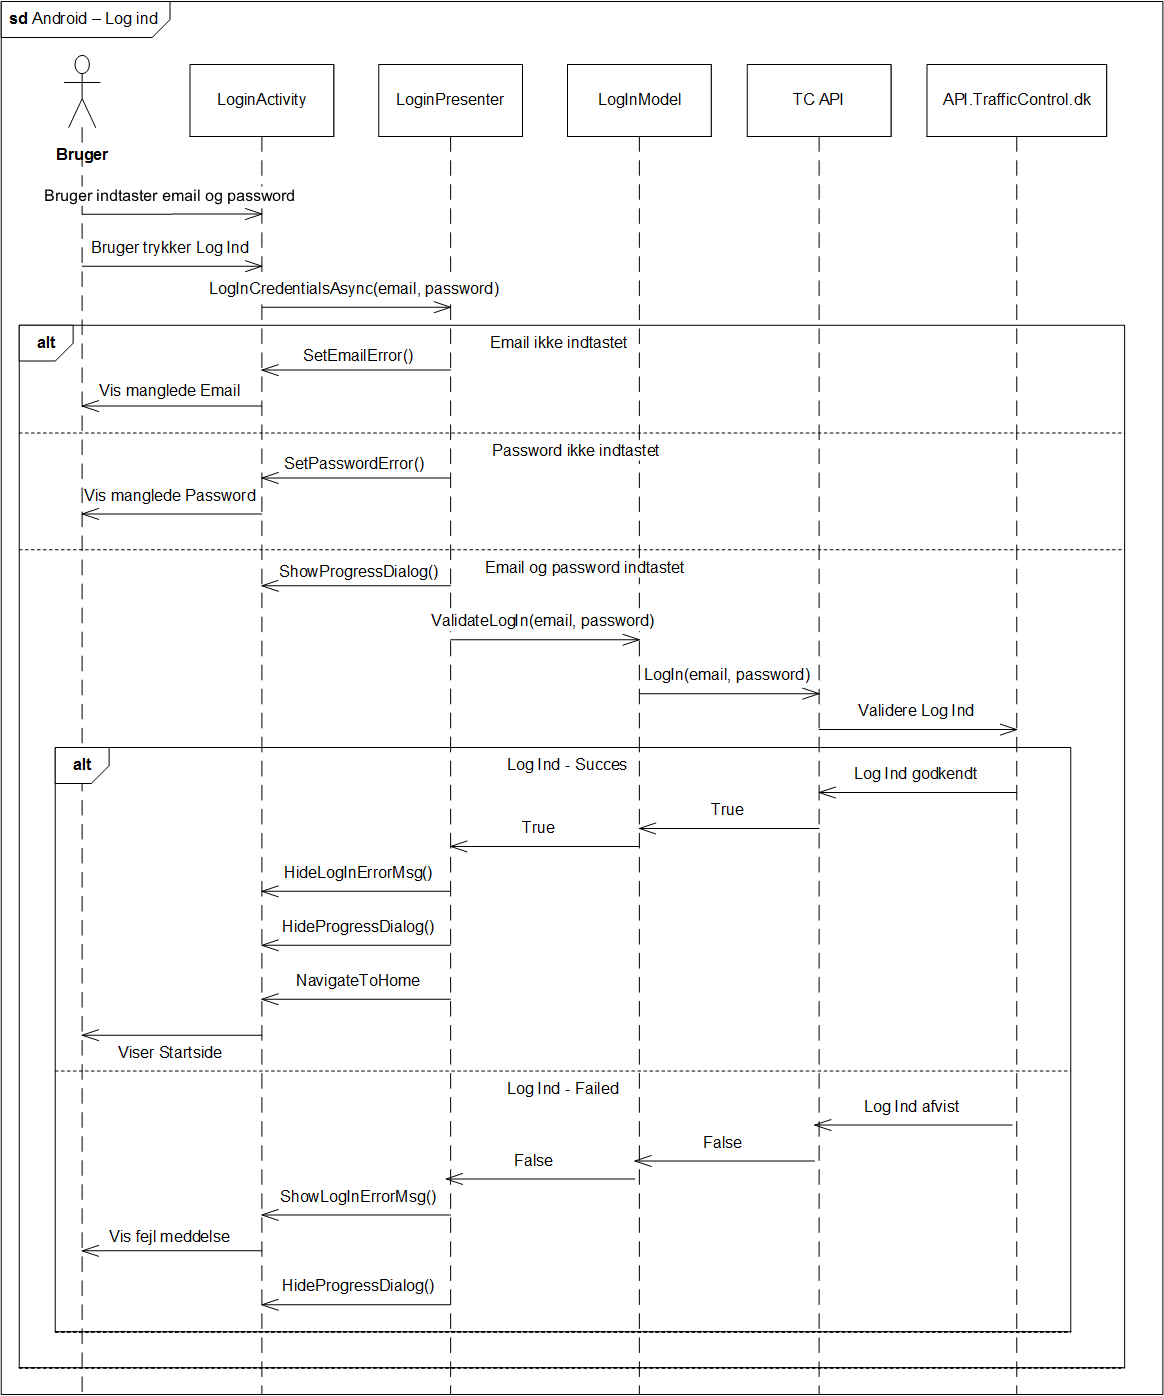
\includegraphics[height=17cm]{SekvensDiagramLogInd}
		\end{center}
		\caption{Sekvens diagram for Log Ind p� Android Applikationen}
		\label{fig:Sekvens diagram for Log Ind Android}
	\end{figure}
	\pagebreak
	
	\subsubsection{Grafisk Bruger Interface}
	Her ses hvordan at Log Ind siden ser ud p� Android Applikationen.
	Det er et meget simpelt design, for at g�re det yderst bruger venligt.
	
			\begin{figure} [h]
				\begin{center}
					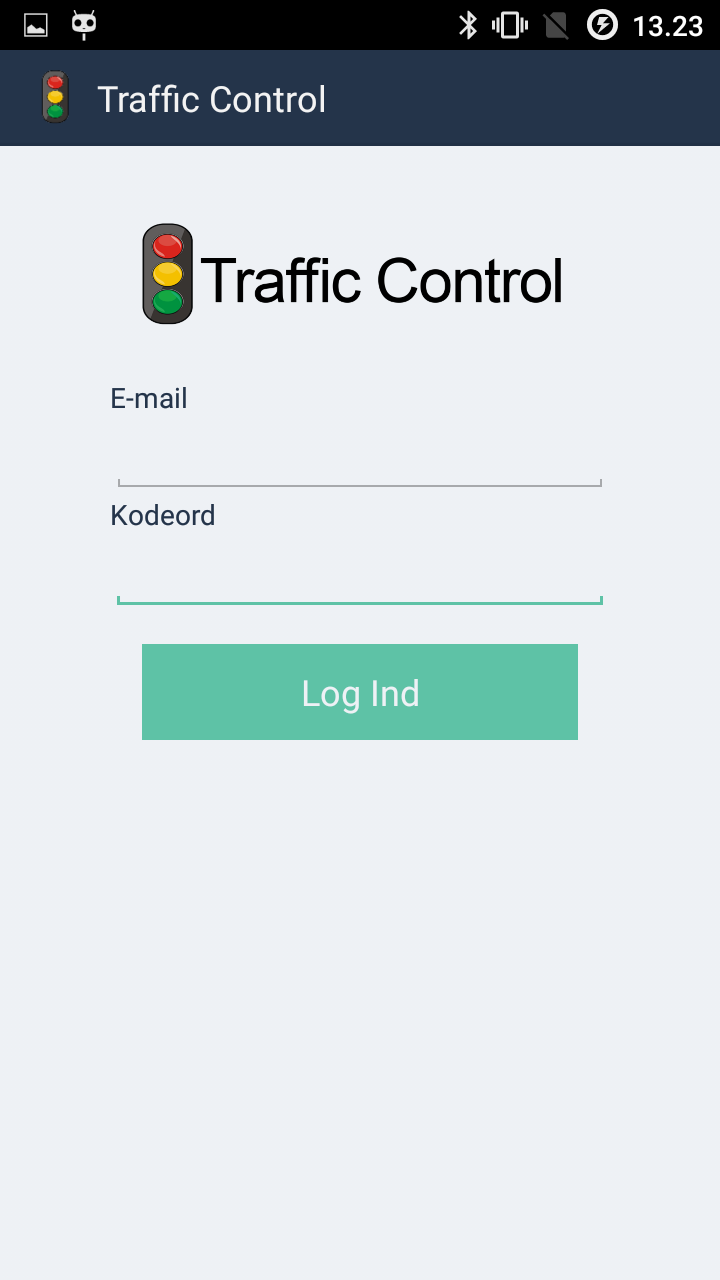
\includegraphics[height=7cm]{AndroidLogIn}
				\end{center}
				\caption{Traffic Control - Log ind}
				\label{fig:Traffic Control - Log ind}
			\end{figure}
	
	\subsubsection{Implementering}
			
	\subsubsection{Test}

	Ja tak\\
	
	\pagebreak
	\subsection{Home page}
	\subsubsection{Design}
	\subsubsection{Grafisk Bruger Interface}
	Hjemsiden er noget mere kompleks end nogle af de andre siger. Dette er fors�gt at gjort simpelt ved ikke at have for mange egenskaber af gangen.
		\begin{figure}[h!]
			\begin{center}
				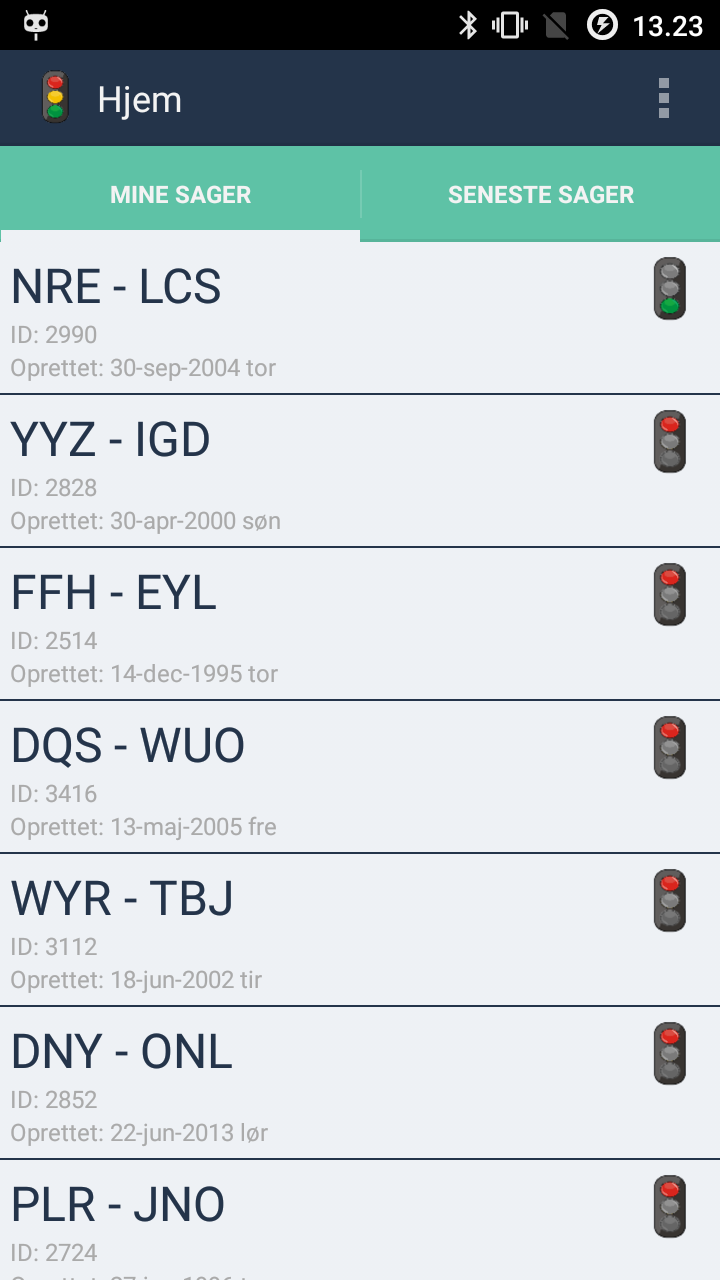
\includegraphics[height=7cm]{AndroidHomePage}
			\end{center}
		\caption{Traffic Control - Home Page}
		\label{fig: Traffic Control - Home Page}
		\end{figure}
		\\
	Hjemsiden indeholder en liste af sager. Trafik lyset ud for sagen viser hvilken status den er i. R�d for lukket, gul for afventer og gr�n for �ben. \\
	Der er to taps hvor man kan v�lge at se alle sager eller om man kun vil se de sager man selv har taget.
		
	\subsubsection{Implementering}
	
	\subsubsection{Test}
	
	Ja tak\\
	\pagebreak
	
	\subsection{Opret bruger}
	\subsubsection{Design}
	Dette afsnit viser et sekvens diagram over Opret bruger forl�bet i Android Applikationen
		\begin{figure} [!ht]
			\begin{center}
				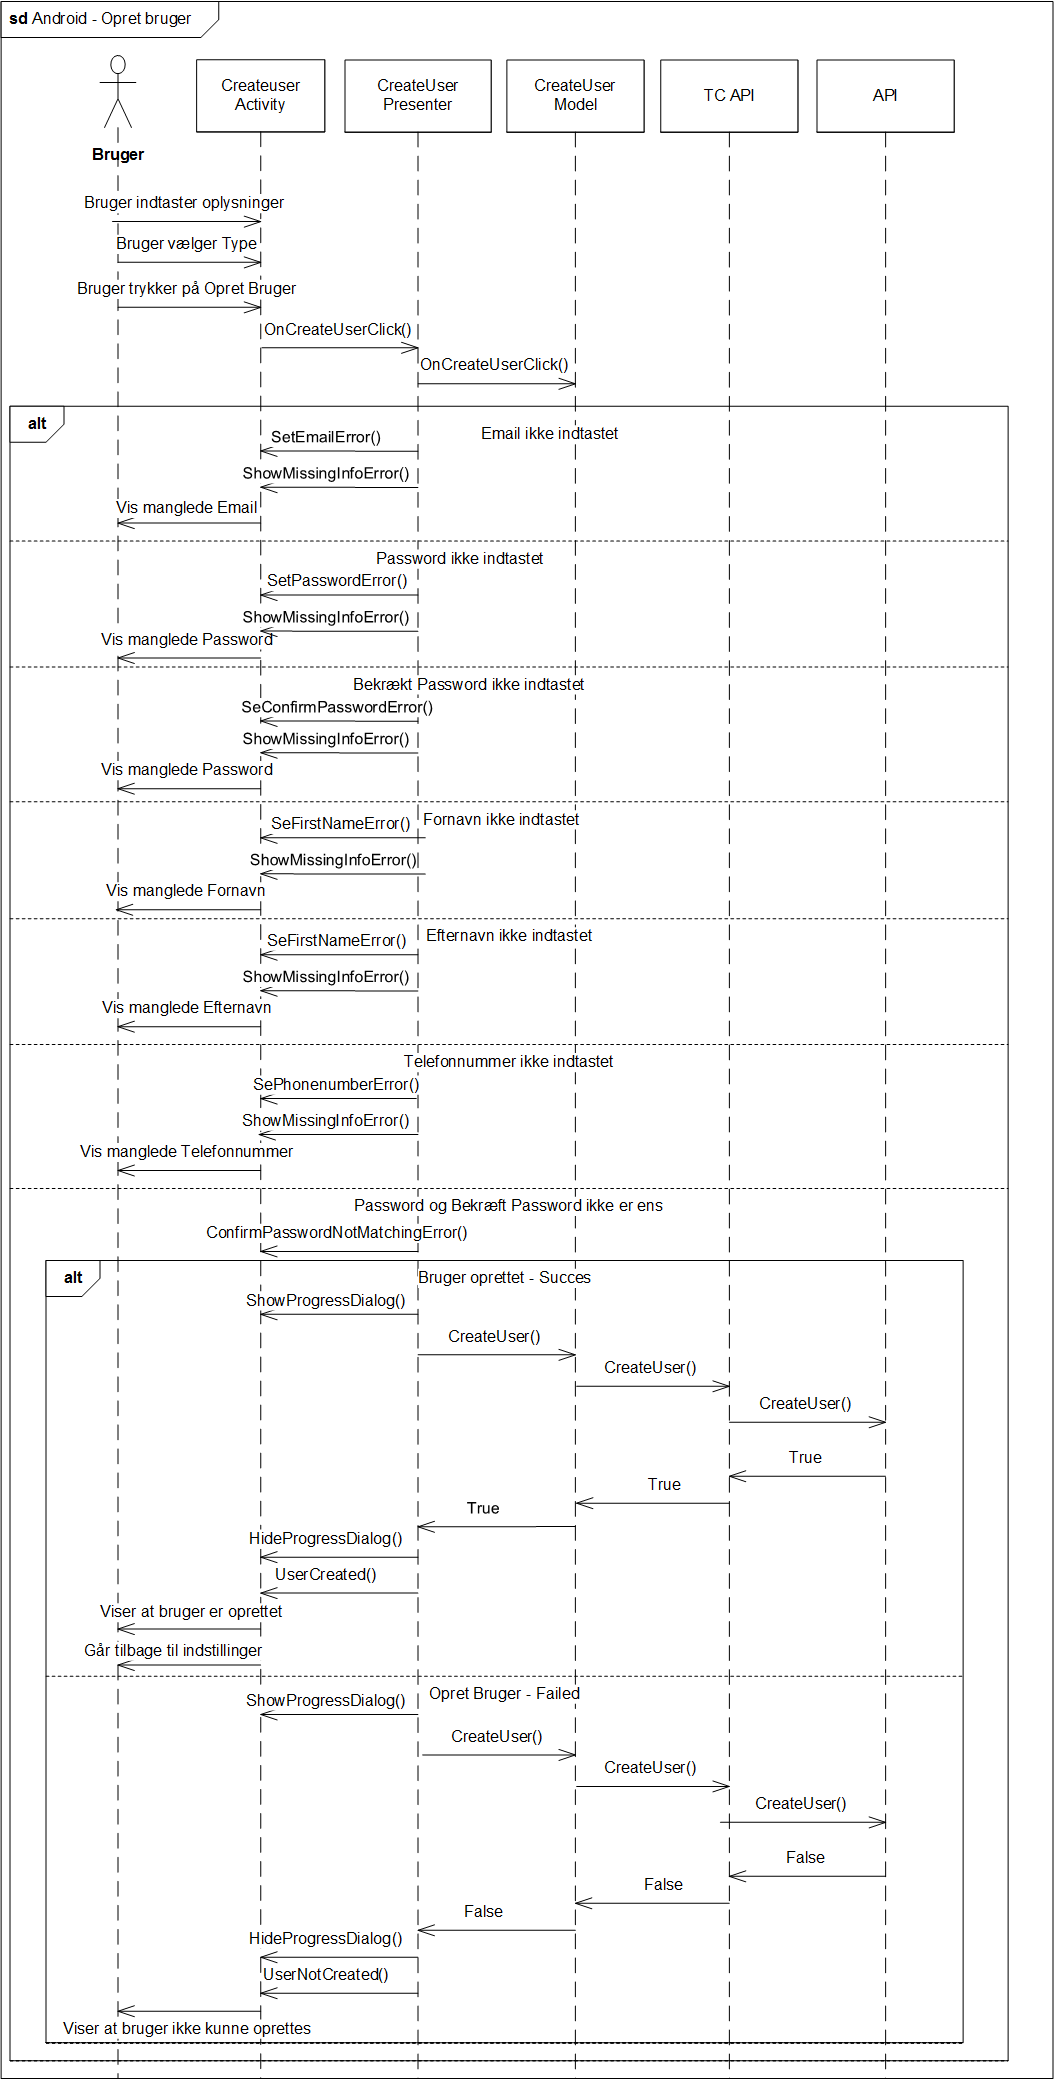
\includegraphics[height=17cm]{OpretBrugerSekvens}
			\end{center}
			\caption{Sekvens diagram for Opret Bruger p� Android Applikationen}
			\label{fig:OpretBrugerSekvens}
		\end{figure}
		\pagebreak
	
	\subsubsection{Grafisk Bruger Interface}
	
		\begin{figure}[!ht]
			\begin{center}
				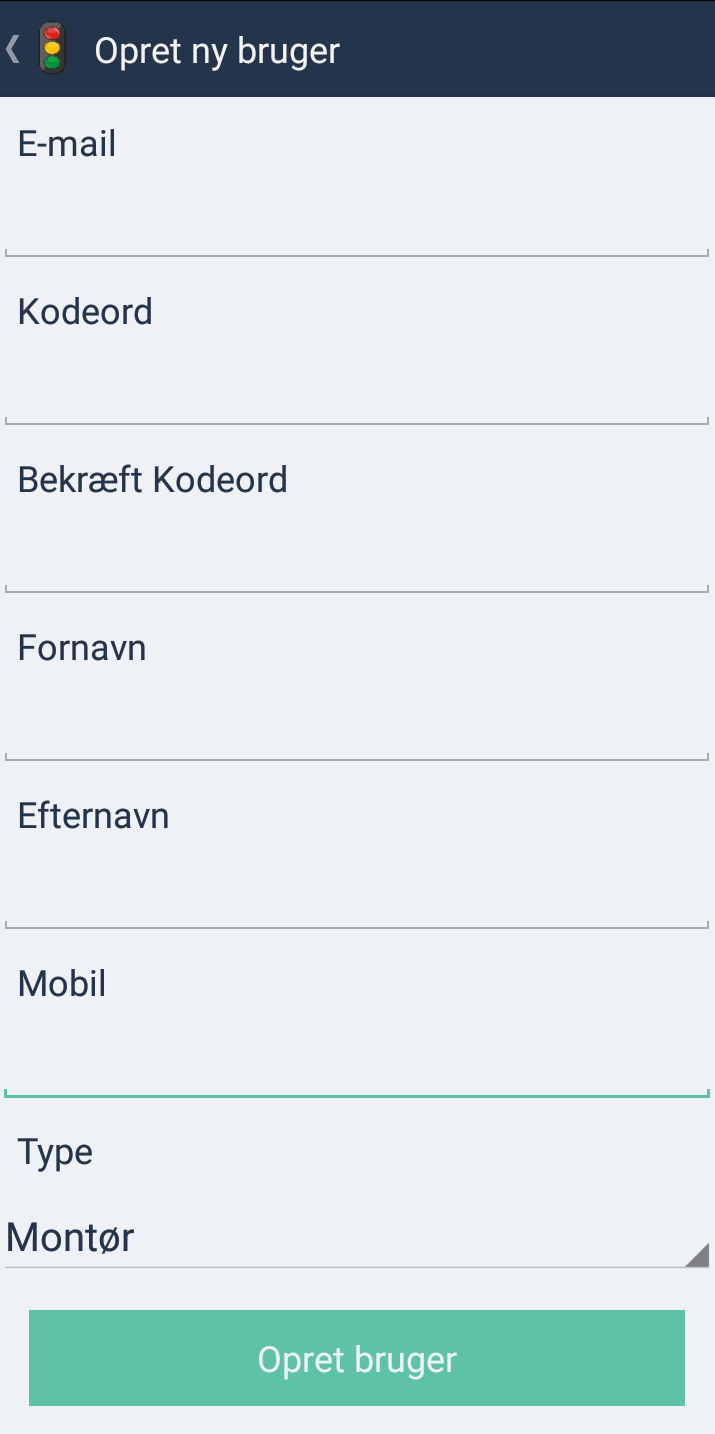
\includegraphics[height=7cm]{AndroidOpretbruger}
			\end{center}
			\caption{Traffic Control - Opret Bruger}
			\label{fig: Traffic Control - Opret Bruger}
		\end{figure}
	
	\noindent Opret bruger siden er igen gjort simpel og nem at arbejde med. Her er lavet felter til alt det info som skal tastes ind om en bruger og til sidst er der lavet en drop down hvor du kan v�lge hvilken type bruger det er.	
\subsubsection{Implementering}

\subsubsection{Test}

Ja tak\\

\end{document}